There are two major activities used in the development of the application: the Main Activity and the Navigation Activity.

The \textbf{Main Activity} displays the menu page, where the user can find a brief description of the application. By tapping the "Go to Navigation" button the user can access the navigation page. This activity is responsible for initializing the necessary dependencies of the Kontatk SDK (BLE beacon API) and managing Bluetooth and Camera Permissions. It checks if the permissions are enabled and prompts the user to activate them if needed.

The \textbf{Navigation Activity} serves as the core part of the application. Its primary responsibility is to enable and verify Bluetooth and GPS Location services.
Subsequently, it instantiates the BLE beacons and QR Code scanners to provide localization and navigation functionalities to the user. As part of its debugging mode, this activity displays updated information about the current region detected and the points of interest (BLE Beacon functionalities). It also shows the updated QR Code point of interest scanned (QR Code functionality). Furthermore, it includes a button to activate the camera view on the screen.

\vfill\null
\columnbreak

\begin{figure}[H]
    \centering
    \begin{subfigure}
        \centering
        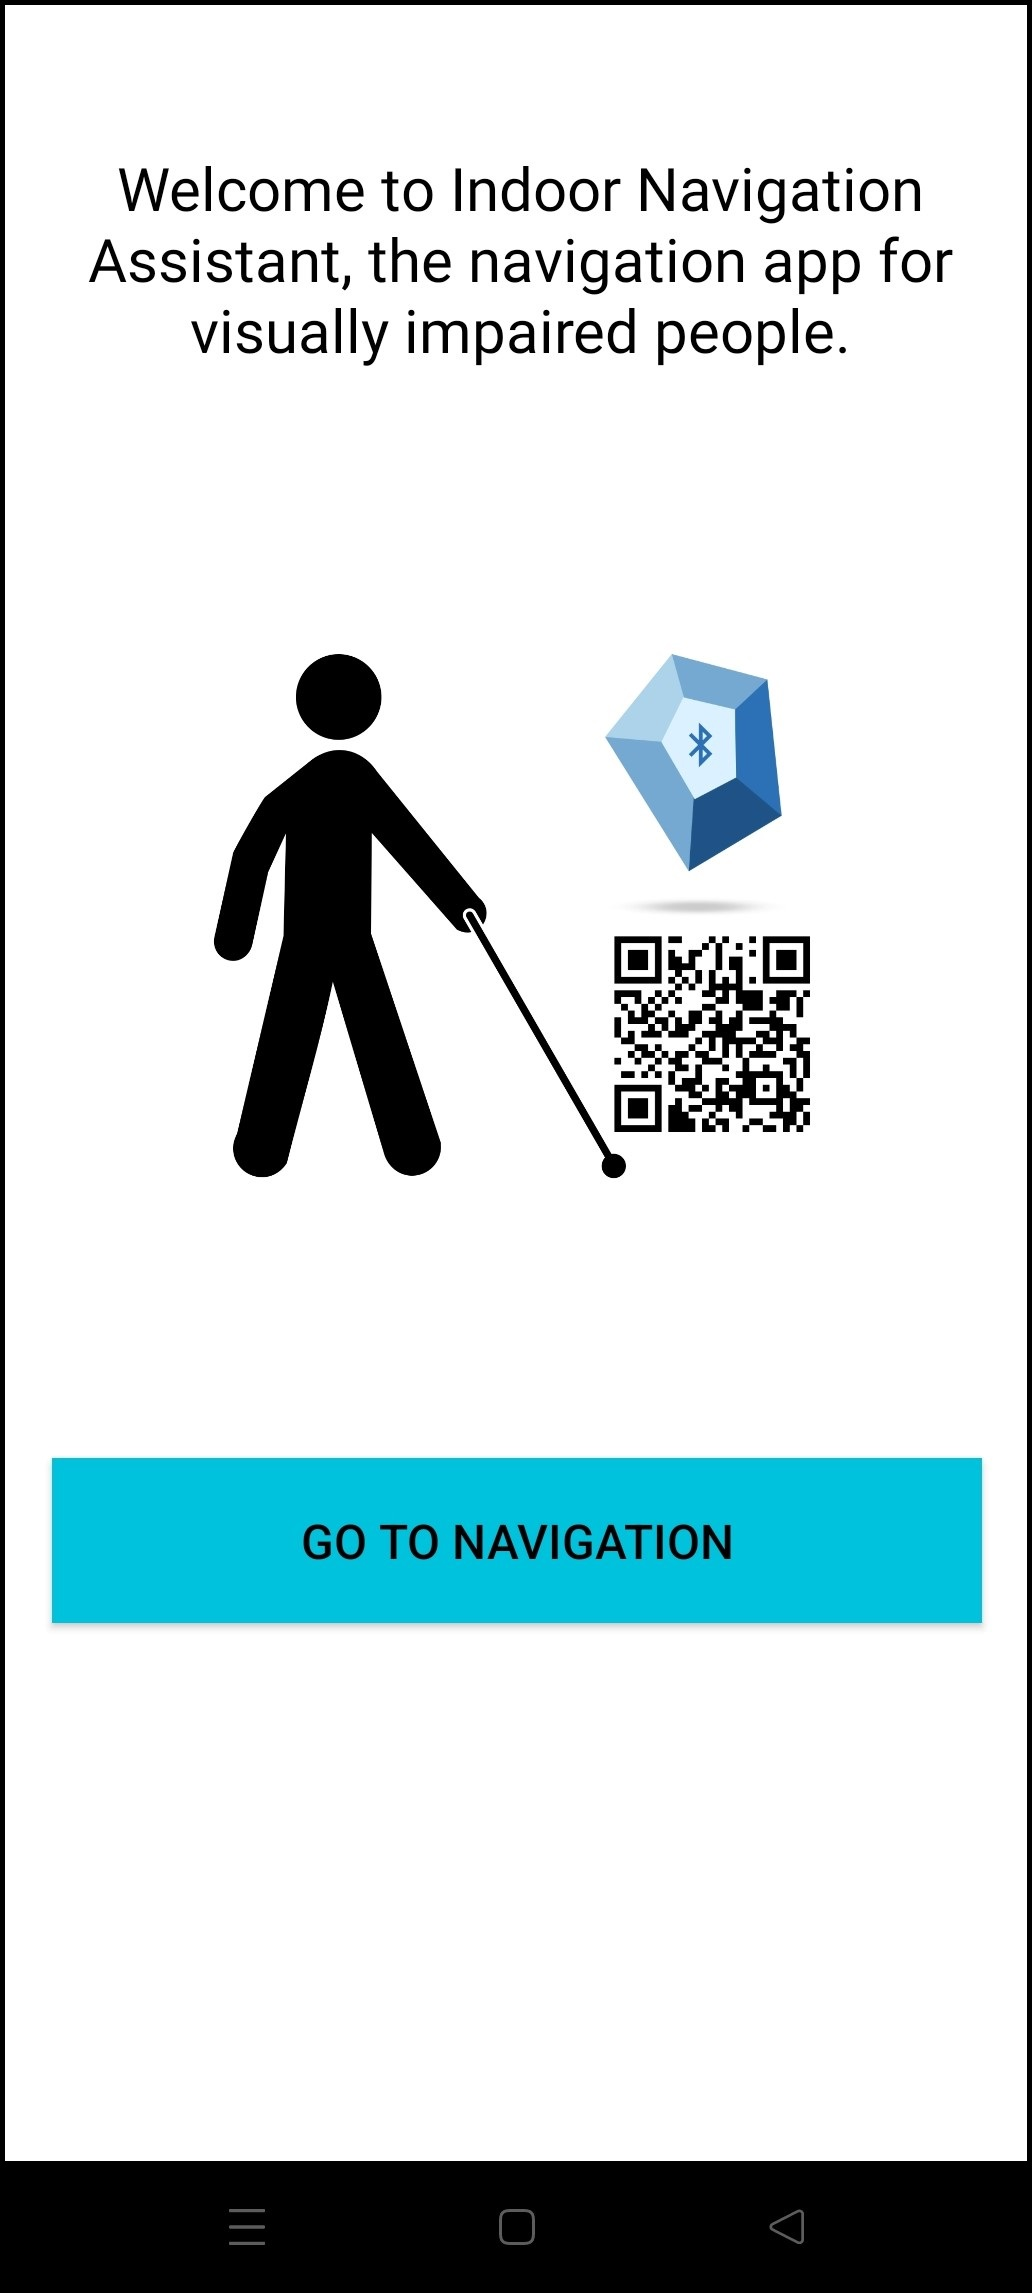
\includegraphics[width=0.2\textwidth]{chapters/architecture/images/main_activity.jpg}
        \label{fig:my_label}
    \end{subfigure}
    \hfill
    \begin{subfigure}
        \centering
        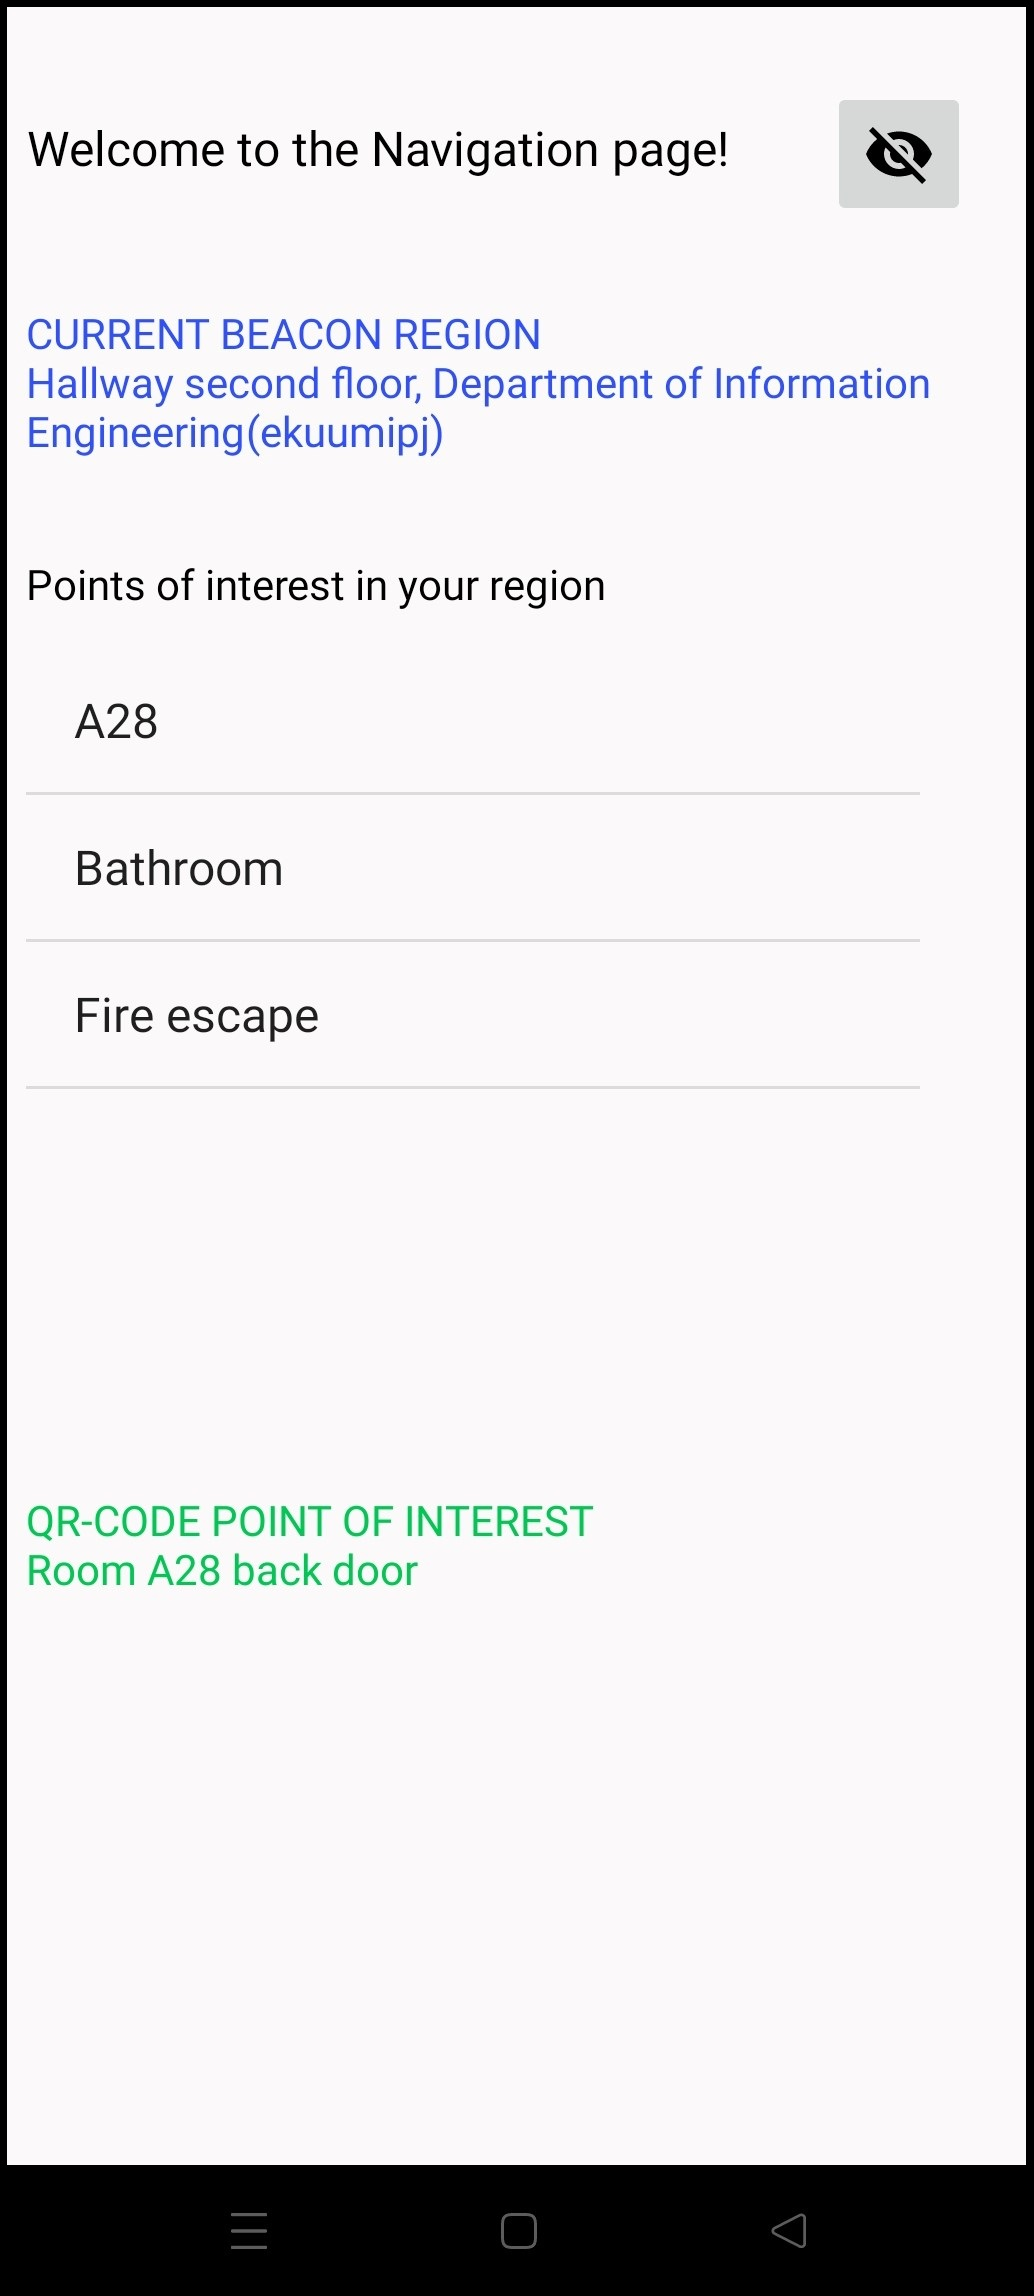
\includegraphics[width=0.2\textwidth]{chapters/architecture/images/navigation_activity.jpg}
    \end{subfigure}
    \caption{Main Activity and Navigation Activity Pages}
\end{figure}
